\clearpage
\section{Summary}

\begin{figure}[ht]
    \begin{center}
        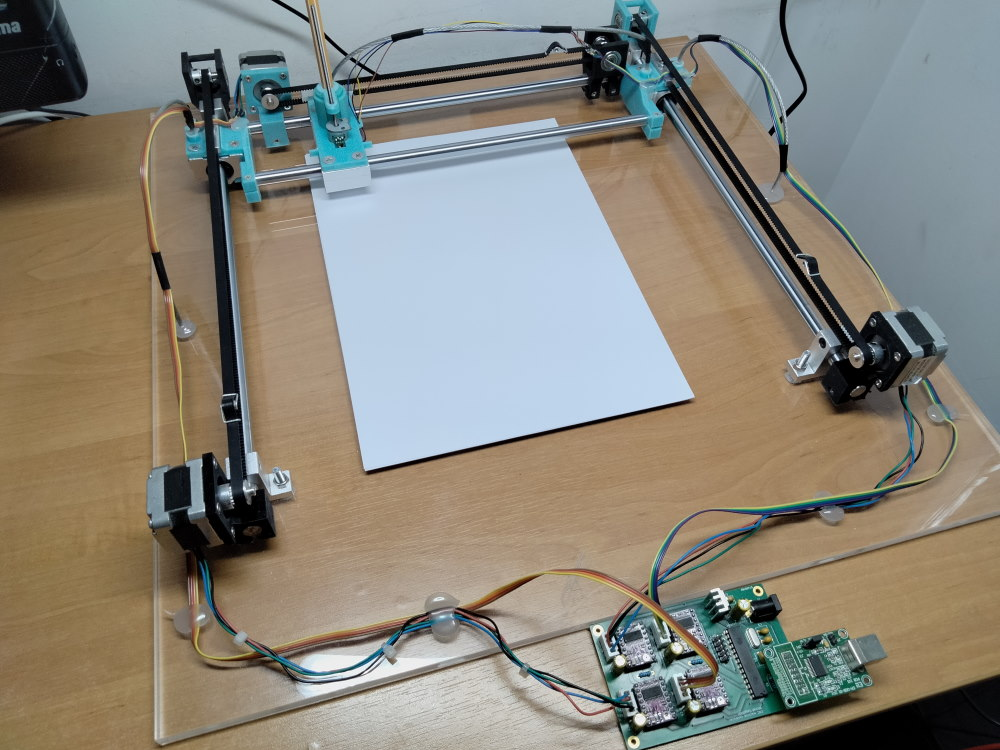
\includegraphics[width=0.8\textwidth]{plotter}
        \caption{The constructed machine.}
    \end{center}
\end{figure}

Prompted by this thesis was the successful construction of a fully functional CNC
machine together with the software needed to operate it. The creation process
involved the design of custom-made mechanical parts, an electronic circuit,
a printed circuit board, and two computer programs, one of which being low-level
microprocessor software and the other a GUI application for desktop computers.

The thesis includes a theoretical introduction to CNC machine design, followed
by a detailed description of the designed device. Provided are circuit
schematics, an overview of the software, detailed descriptions of algorithms
and data structures, illustrations of the user interface, and photographs
demonstrating the capabilities of the machine.

The designed solution meets project requirements. It is easy to use and enables
a non\-technical user to operate a CNC machine without prior training. In many
respects, however, it is still but a proof-of-concept. The firmware is greatly
limited in functionality and supports only a small subset of G-code. The bitmap
tracing feature produces only straight lines at predetermined angles.
3D-printed parts have high tolerances and produce visible imperfections.
Nonetheless, these are not critical problems, and resolving them may be a
suitable subject for a later thesis.
